\documentclass[11pt]{article}
\usepackage[margin=1in]{geometry}
\usepackage[T1]{fontenc}
\usepackage{lmodern}
\usepackage{amsmath,amssymb,amsthm,mathtools}
\usepackage{bm}
\usepackage{booktabs}
\usepackage{graphicx}
\usepackage{xcolor}
\usepackage{algorithm}
\usepackage{algpseudocode}
\usepackage{hyperref}
\usepackage[numbers,sort&compress]{natbib}
\usepackage{enumitem}
\usepackage{caption}
\usepackage{multirow}
\usepackage[section]{placeins}
\usepackage{microtype}
\emergencystretch=1.5em
\hypersetup{colorlinks=true,linkcolor=blue!50!black,citecolor=blue!50!black,urlcolor=blue!50!black}

\newtheorem{theorem}{Theorem}
\newtheorem{proposition}{Proposition}
\newtheorem{lemma}{Lemma}
\newtheorem{corollary}{Corollary}
\theoremstyle{definition}
\newtheorem{definition}{Definition}
\newtheorem{assumption}{Assumption}
\theoremstyle{remark}
\newtheorem{remark}{Remark}

\renewcommand{\thesection}{S\arabic{section}}
\renewcommand{\thetheorem}{S\arabic{theorem}}
\renewcommand{\theproposition}{S\arabic{proposition}}
\renewcommand{\thelemma}{S\arabic{lemma}}
\renewcommand{\thecorollary}{S\arabic{corollary}}
\renewcommand{\thedefinition}{S\arabic{definition}}
\renewcommand{\theassumption}{S\arabic{assumption}}
\renewcommand{\thetable}{S\arabic{table}}
\renewcommand{\thefigure}{S\arabic{figure}}
\renewcommand{\theequation}{S\arabic{equation}}
\renewcommand{\thealgorithm}{S\arabic{algorithm}}

\newcommand{\R}{\mathbb{R}}
\newcommand{\E}{\mathbb{E}}
\newcommand{\cP}{\mathcal{P}}
\newcommand{\tr}{\operatorname{tr}}
\newcommand{\op}{\mathrm{op}}
\newcommand{\rhohat}{\hat\rho}
\DeclareMathOperator*{\argmax}{arg\,max}

\title{Supplementary Material for\\ ``DisCo-CFL: Calibrated, Fair and Explainable Clustered Federated Learning via Disattenuated Class-Conditional Gradient Signatures''}
\author{Quang-Vinh Dang\\ British University Vietnam, Hung Yen, Vietnam\\ \texttt{vinh.dq4@buv.edu.vn}}
\date{}

\begin{document}
\maketitle

\noindent This supplement contains the full definitions and statements (Section~\ref{app:defs}), all proofs (Section~\ref{app:proofs}), the Lean~4 formalisation (Section~\ref{app:lean}), and additional experimental details and results (Section~\ref{app:results}). Results carry the prefix ``S''. They correspond to the main paper as follows: Proposition~\ref{prop:inv} is Proposition~1; Lemma~\ref{lem:pop} and Theorem~\ref{thm:conc} together form Theorem~1; Theorems~\ref{thm:rec} and~\ref{thm:lb} are Theorems~2 and~3; Corollary~\ref{cor:sc} is Corollary~1; Proposition~\ref{prop:dp} is Proposition~2; Propositions~\ref{prop:expl} and~\ref{prop:pc} together form Proposition~3.

\section{Definitions and full statements}\label{app:defs}
\begin{definition}[Concept equivalence and conflicts]\label{def:concept}
Clients $i$ and $j$ \emph{conflict on class} $c\in S_i\cap S_j$ if $\cP_i(X\mid Y=c)\neq\cP_j(X\mid Y=c)$. They are \emph{compatible} if they conflict on no shared class. Clients belong to $K$ latent concept groups $G_1,\dots,G_K$: $\cP_i(X\mid Y=c)=\cP^{(k)}(X\mid Y=c)$ for $i\in G_k$.
\end{definition}

\subsection{Method definitions}\label{sec:method}
\subsubsection{Class-conditional gradient signatures (client side)}
After $T_0$ warm-up rounds of FedAvg the server broadcasts a reference model $w$ and the seed of a count-sketch $\Phi:\R^d\to\R^p$~\citep{charikar2002countsketch,weinberger2009hashing} ($p=1024$). For a sample $(x,c)$ let $g(x,c)=\Phi\nabla_w\ell(w;x,c)\in\R^p$. For every class $c\in S_i$ the client randomly splits its class-$c$ samples into halves $A_i^c,B_i^c$ of size $h_i^c$ and sends
\[ a_i^c=\frac1{h_i^c}\sum_{s\in A_i^c}g(x_s,c),\qquad b_i^c=\frac1{h_i^c}\sum_{s\in B_i^c}g(x_s,c). \]
Per-sample sketched gradients are clipped to a shared norm $C_{\rm clip}$ ($0.5$ in all experiments) before averaging. Per-sample gradients at a trained reference model are extremely heavy-tailed: in our Fashion-MNIST runs the median norm is $0.08$ and the 99th percentile about $23$, so a handful of hard examples would otherwise dominate a class signature. The expected clipped gradient is still a functional of $\cP_i(X\mid Y=c)$, so invariance is preserved, and clipping makes per-sample signatures bounded, hence sub-Gaussian as required by Assumption~\ref{ass:noise}. The upload happens \emph{once} and costs $2p|S_i|\le 2pC$ floats, independent of the model size $d$. For our small CNN ($d\approx4.7\times10^4$) this is comparable to one model upload; for realistic models with $d\gg 2pC$ it is negligible. For differential privacy (Proposition~\ref{prop:dp}), Gaussian noise is added to each clipped half-mean.

\subsubsection{Disattenuated similarity (server side)}
Let $m_i^c=(a_i^c+b_i^c)/2$. The split-half reliability and its Spearman--Brown extension to the full mean are
\begin{equation}\label{eq:rel}
r_i^c=\cos(a_i^c,b_i^c),\qquad R_i^c=\frac{2r_i^c}{1+r_i^c}\quad(R_i^c:=0 \text{ if } r_i^c\le 0).
\end{equation}
The calibrated similarity of $i$ and $j$ on class $c$ is
\begin{equation}\label{eq:disatt}
\rhohat_{ij}^c=\operatorname{clip}_{[-1,1]}\!\left(\frac{\cos(m_i^c,m_j^c)}{\sqrt{R_i^cR_j^c}}\right),\qquad W_{ij}^c=R_i^cR_j^c,
\end{equation}
where $W_{ij}^c$ is the evidence weight. In the population version of~\eqref{eq:disatt} the attenuation factors cancel exactly (Lemma~\ref{lem:pop}), so $\rhohat$ targets $\rho_{ij}^c=\cos(\mu_i^c,\mu_j^c)$, the cosine between expected class-conditional gradients, whatever the sample sizes and noise levels.

\subsubsection{Threshold clustering with bottleneck linkage}
For two sets of clients $A,B$ and a class $c$, let $\mathrm{num}^c_{AB}=\sum_{i\in A,j\in B}W_{ij}^c\rhohat_{ij}^c$ and $\mathrm{den}^c_{AB}=\sum W_{ij}^c$. The linkage is
\begin{equation}\label{eq:link}
L(A,B)=\min_{c}\;\frac{\mathrm{num}^c_{AB}+\lambda}{\mathrm{den}^c_{AB}+\lambda}\qquad\text{if }\textstyle\sum_c\mathrm{den}^c_{AB}\ge e_{\min},\ \text{else }-\infty.
\end{equation}
The \emph{minimum} over classes encodes the definition of concept equivalence: two groups share a concept only if every class-conditional gradient agrees, so a label swap affecting two of ten classes is not averaged away. The shrinkage $\lambda$ pulls classes with little evidence towards $1$ (``no evidence of a difference''). Starting from singletons, the server repeatedly merges, among the pairs with $L\ge\tau$, the pair with the \emph{largest shared evidence}. Well-supported groups therefore form first, and clients that carry little information on the discriminative classes join them afterwards instead of bridging different groups. Merging stops when no pair reaches $\tau$. Because the scale is calibrated, $\tau$ has a fixed meaning: we use $\tau=0.8$ in \emph{all} experiments, with $\lambda=0.5$. Clients with total reliability $\sum_c R_i^c<0.3$ are \emph{low-evidence}: they are excluded from shaping clusters and attached to their most similar cluster afterwards. A singleton cluster is attached to its closest cluster unless the evidence \emph{significantly} separates them (upper confidence bound below $\tau$), in which case it is kept and flagged as \emph{anomalous}. Each cluster then runs FedAvg from $w$. Algorithm~\ref{alg:disco} summarises the procedure.

\begin{algorithm}[t]
\caption{DisCo-CFL}\label{alg:disco}
\begin{algorithmic}[1]
\State Warm-up: $T_0$ rounds of FedAvg on all clients $\to$ reference model $w$; broadcast $w$ and sketch seed
\For{each client $i$ \textbf{in parallel}} \Comment{once}
 \For{$c\in S_i$} split class-$c$ samples into halves, send $(a_i^c,b_i^c)$ (per-sample clipped; noised if DP) \EndFor
\EndFor
\State Server: $R_i^c$ by~\eqref{eq:rel}; $\rhohat^c_{ij},W^c_{ij}$ by~\eqref{eq:disatt}
\State Clusters $\gets$ singletons of clients with enough evidence
\While{$\exists A,B$ with $L(A,B)\ge\tau$} merge the eligible pair with the largest $\sum_c\mathrm{den}^c_{AB}$; log it \EndWhile
\State Attach low-evidence clients and non-significant singletons; flag anomalies
\State Output clusters, certificates, explanations, audit log; run FedAvg within each cluster from $w$
\end{algorithmic}
\end{algorithm}

\subsubsection{Inference: prior-corrected cluster models}\label{sec:pc}
Clusters are built so that their members share class-conditionals but may have very different label proportions. By Bayes' rule, the posterior of client $i$ is obtained from that of its cluster $k$ by re-weighting the prior (Proposition~\ref{prop:pc}). Client $i$ therefore predicts with
\begin{equation}\label{eq:pc}
\hat y(x)=\argmax_y\ \big[f_k(x)_y+\log\hat p_i(y)-\log\hat p_k(y)\big],
\end{equation}
where $f_k$ are the logits of the cluster model, $\hat p_i$ is the client's own (smoothed) label distribution, and $\hat p_k$ is the label distribution of the cluster's training data. The latter is a sum of label counts that the server can obtain by secure aggregation, so no individual histogram is revealed. This correction~\citep{lipton2018labelshift,menon2021logit} costs nothing at training time. It is exactly what concept-level clustering calls for: label skew is handled by the prior, not by more clusters. In the experiments we apply the same correction to \emph{every} method, for a fair comparison.

\subsubsection{Transparency and accountability outputs}\label{sec:outputs}
\begin{itemize}[leftmargin=*,itemsep=1pt]
\item \textbf{Class-level explanations.} For every pair of clusters the server reports the pooled per-class similarity and the set of \emph{divergent classes} $\hat D_{AB}=\{c:\rho^c_{AB}<\tau\}$.
\item \textbf{Heterogeneity diagnosis.} If $\hat D_{AB}$ contains every shared class, the server reports a global (feature-level) concept shift; if it is a strict subset, a class-specific shift on the listed classes; if $\hat K=1$, it reports that the heterogeneity is explained by target and quantity skew only.
\item \textbf{Assignment certificates.} Each client receives its bottleneck similarity to its own cluster and to the closest other cluster, the bottleneck classes, and standard errors from the spread over member pairs. A certificate is \emph{confident} if $s_{\rm own}-z\,\mathrm{se}\ge\tau$ and $s_{\rm other}+z\,\mathrm{se}<\tau$ ($z=2$); otherwise it is \emph{uncertain} or \emph{low-evidence}.
\item \textbf{Audit log} of every merge (members, linkage, bottleneck class, evidence) and of every attachment or anomaly decision, so that each grouping can be traced and contested.
\item \textbf{Newcomers} compute their signature at the same frozen $w$ and join the cluster with the highest bottleneck similarity if it reaches $\tau$. Otherwise they are reported as a \emph{novel concept}.
\end{itemize}


\subsection{Full statements}\label{sec:theory}
Proofs are in Section~\ref{app:proofs}; their deterministic parts are formalised in Lean~4 (Section~\ref{app:lean}). Write $\mu_i^c=\E_{x\sim\cP_i(X\mid Y=c)}[g(x,c)]$ and $a_i^c=\|\mu_i^c\|^2$.

\begin{proposition}[Invariance]\label{prop:inv}
$\mu_i^c$ is a functional of $\cP_i(X\mid Y=c)$ only. Consequently, for compatible clients $\rho^c_{ij}=1$ on every shared class, whatever their label proportions $\cP_i(Y),\cP_j(Y)$ and sample sizes $n_i,n_j$.
\end{proposition}

\begin{assumption}[Noise]\label{ass:noise}
Per-sample signatures are $g=\mu_i^c+\Sigma^{1/2}z$ with independent $z$ having independent, zero-mean, unit-variance, $K_0$-sub-Gaussian coordinates. Let $\sigma^2=\tr\Sigma$, and define the effective ranks $r_s=\tr\Sigma/\|\Sigma\|_{\op}$ and $r_e=(\tr\Sigma)^2/\|\Sigma\|_F^2$.
\end{assumption}
\begin{assumption}[Identifiability]\label{ass:sep}
If $i,j$ conflict on $c$, then $\rho^c_{ij}\le1-\Delta$ for some $\Delta\in(0,1]$.
\end{assumption}
For a pair and a class let $h=\min(h_i^c,h_j^c)$, $a=\min(a_i^c,a_j^c)$, and let $\kappa=\sigma^2/(ah)$ be the inverse signal-to-noise ratio of a half-mean.

\begin{lemma}[Exact calibration at the population level]\label{lem:pop}
Replacing each inner product and squared norm in~\eqref{eq:rel}--\eqref{eq:disatt} by its expectation gives exactly $\rho_{ij}^c$.
\end{lemma}

\begin{theorem}[Concentration]\label{thm:conc}
Under Assumption~\ref{ass:noise}, let $\kappa\le1$ and $\delta\in(0,1)$. There are constants $c_0,C_1$ depending only on $K_0$ such that, if
\[
\eta:=\Big(\sqrt{\kappa/r_s}+\kappa/\sqrt{r_e}\Big)\sqrt{\log(12/\delta)}\;\le\; c_0,
\]
then with probability at least $1-\delta$
\[
|\rhohat_{ij}^c-\rho_{ij}^c|\le C_1\,\eta,
\qquad
|R_i^c-R_i^{c,\star}|\le C_1\eta,
\qquad
R_i^{c,\star}:=\frac{a_i^c}{a_i^c+\sigma^2/(2h_i^c)}.
\]
In contrast, the raw cosine $\cos(m_i^c,m_j^c)$ converges to $\rho^c_{ij}\sqrt{R_i^{c,\star}R_j^{c,\star}}$. It is biased towards $0$ by a factor that depends on the sample sizes.
\end{theorem}

\begin{theorem}[Safety, maximality, recovery]\label{thm:rec}
Let $\gamma=\min(1-\tau,\ \tau-1+\Delta)>0$ and $w_0:=2\lambda(1-\tau)/\gamma$. Suppose that all estimates satisfy $|\rhohat^c_{ij}-\rho^c_{ij}|\le\gamma/2$ (event $\mathcal E$) and that every pair conflicting on a class $c$ has evidence $W^c_{ij}>w_0$. Then the merging phase of Algorithm~\ref{alg:disco}, in any merge order, satisfies:
\begin{enumerate}[label=(\alph*),itemsep=0pt]
\item \emph{Safety:} no cluster ever contains two conflicting clients.
\item \emph{Maximality:} any two output clusters with shared evidence $\ge e_{\min}$ contain a conflicting pair, so no two output clusters can be merged without mixing concepts.
\item \emph{Exact recovery:} if every client holds every class on which some groups differ, and every pair of clients shares evidence $\ge e_{\min}$, the output partition equals $\{G_1,\ldots,G_K\}$; in particular $\hat K=K$.
\end{enumerate}
\end{theorem}

\begin{corollary}[Sample complexity and minority fairness]\label{cor:sc}
Under Assumptions~\ref{ass:noise}--\ref{ass:sep}, let $\gamma\le1/3$ and $\lambda<\gamma/(8(1-\tau))$. The conclusions of Theorem~\ref{thm:rec} hold with probability at least $1-\delta$ as soon as every reported half size satisfies
\begin{equation}\label{eq:hstar}
h\;\ge\;h^\star:=C_2\,\frac{\sigma^2}{a}\,
\max\Big\{\frac{\mathsf L}{r_s\,\gamma^2},\ \frac{\sqrt{\mathsf L}}{\sqrt{r_e}\,\gamma},\ 1\Big\},
\qquad \mathsf L:=\log\frac{12N^2C}{\delta}.
\end{equation}
$h^\star$ does not depend on the sizes of the groups $|G_k|$, on the number of clients per group, or on the other clients' dataset sizes (apart from $\log N$). A concept group made of a \emph{single} client is recovered under the same condition as a group of a hundred.
\end{corollary}

\begin{theorem}[Minimax lower bound]\label{thm:lb}
Let $\xi\sim\mathcal N(0,\Sigma)$ and $\|\mu\|^2=a$. For any test that decides from $n$ per-sample signatures of client $j$, even when $\mu_i$ is known exactly, whether $\rho_{ij}=1$ or $\rho_{ij}=1-\Delta$, the worst-case error probability is at least
\[
\tfrac14\exp\!\big(-n\,a\,\Delta\,r_s/\sigma^2\big).
\]
Error at most $\delta$ therefore requires
\[
n\;\ge\;\frac{\sigma^2}{a\,r_s\,\Delta}\,\log\frac1{4\delta}.
\]
\end{theorem}
With $\tau$ in the middle of the admissible interval ($\gamma=\Delta/2$), the leading term of~\eqref{eq:hstar} is
\[
O\!\left(\frac{\sigma^2\log(N^2C/\delta)}{a\,r_s\,\Delta^2}\right).
\]
The upper and lower bounds therefore agree in their dependence on noise $\sigma^2$, signal $a$ and effective rank $r_s$, and differ by a factor $1/\Delta$ and a $\log N$ term.

\begin{proposition}[Differential privacy and its cost]\label{prop:dp}
Suppose each released half-mean is
\[
\frac1h\sum_{s}\operatorname{clip}_{C_{\rm clip}}(g_s)+\xi_{\rm dp},
\qquad
\xi_{\rm dp}\sim\mathcal N\!\big(0,(2\sigma_{\rm dp}C_{\rm clip}/h)^2I_p\big).
\]
(i) Every sample enters exactly one released vector, whose replace-one sensitivity is $2C_{\rm clip}/h$. The signature is therefore $(\varepsilon,\delta)$-DP with respect to replacing one record by another of the same label, with $(\varepsilon,\delta)$ given by the analytic Gaussian mechanism~\citep{balle2018analytic} at noise multiplier $\sigma_{\rm dp}$ (parallel composition). The class support $S_i$ is released in the clear.
(ii) The DP noise is independent of sampling noise. Lemma~\ref{lem:pop} therefore still holds, and Theorem~\ref{thm:conc} applies with the half-mean covariance $\Sigma/h+(2\sigma_{\rm dp}C_{\rm clip}/h)^2I_p$. The recovery guarantee then requires, in addition to~\eqref{eq:hstar},
\[
h\;\gtrsim\;\sigma_{\rm dp}C_{\rm clip}\left(\frac{\sqrt{\mathsf L}}{\sqrt a\,\gamma}+\frac{p^{1/4}\,\mathsf L^{1/4}}{\sqrt{a\gamma}}\right),
\]
so the per-class sample size grows linearly in $\sigma_{\rm dp}\propto1/\varepsilon$.
(iii) Without disattenuation, the raw cosine tends to $\rho\,\sqrt{R_iR_j}$ with
\[
R\approx\frac{a}{a+2p\,\sigma^2_{\rm dp}C_{\rm clip}^2/h^2}.
\]
Unless $h\gg\sqrt p\,\sigma_{\rm dp}C_{\rm clip}/\sqrt a$, same-concept clients look unrelated.
\end{proposition}

\begin{proposition}[Explanation fidelity]\label{prop:expl}
On $\mathcal E$, if two output clusters $A,B$ have pooled evidence $\mathrm{den}^c_{AB}>w_0$ on a class $c$, then $c\in\hat D_{AB}$ if and only if $\cP_A(X\mid Y=c)\neq\cP_B(X\mid Y=c)$. The reported divergent classes are exactly the classes on which the two concepts differ.
\end{proposition}

\begin{proposition}[Prior correction is Bayes-optimal within a concept cluster]\label{prop:pc}
Let cluster $k$ consist of concept-equivalent clients with pooled distribution $\cP_k(X,Y)=\cP_k(Y)\cP(X\mid Y)$, and let $q_k(y\mid x)$ be its Bayes posterior. For every member $i$, $\cP_i(y\mid x)\propto q_k(y\mid x)\,\cP_i(y)/\cP_k(y)$. Hence~\eqref{eq:pc} with the true priors and $f_k=\log q_k$ is the Bayes-optimal classifier of client $i$. No clustering finer than concept equivalence can reduce the Bayes risk of any member.
\end{proposition}

\begin{remark}[Scope of the guarantees]
Theorem~\ref{thm:rec} covers the merging phase. The attachment of low-evidence clients and of non-significant singletons is a fairness heuristic: it avoids training a client alone because of noise, may violate safety when evidence is weak, and is logged in the audit trail. Corollary~\ref{cor:sc} asks for a small $\lambda$ so that a single pair of clients carries enough evidence. Our default $\lambda=0.5$ is larger. It makes the method more conservative about splitting on thin evidence, and merges quickly happen between clusters whose pooled evidence far exceeds $w_0$. Table~\ref{tab:lambda} reports the sensitivity to $\lambda$, including values that satisfy the corollary.
\end{remark}



\section{Proofs}\label{app:proofs}
Throughout, $C,C_1,C_2,\dots$ and $c_0$ denote constants that depend only on the sub-Gaussian constant $K_0$ and may change from line to line. We fix a class $c$ and drop it from the notation when no confusion arises. Statements whose deterministic core is machine-checked in Lean~4 are marked with the name of the corresponding Lean theorem (Section~\ref{app:lean}).

\subsection{Proof of Proposition~\ref{prop:inv}}
The reference model $w$, the sketch $\Phi$ and the label $c$ are the same for all clients, so
\[
\mu_i^c=\int \Phi\,\nabla_w\ell(w;x,c)\;d\cP_i(x\mid Y=c)
\]
is determined by $\cP_i(X\mid Y=c)$ alone. Neither the proportion $\cP_i(Y=c)$ nor the number of samples enters. If $i$ and $j$ are compatible, then $\cP_i(X\mid Y=c)=\cP_j(X\mid Y=c)$ on each shared class, hence $\mu_i^c=\mu_j^c$ and $\rho^c_{ij}=1$. Per-sample clipping is applied identically by all clients, so the same holds for the expected clipped signature. \qed

\subsection{Proof of Lemma~\ref{lem:pop}}
Write the half-means as $a_i=\mu_i+\zeta_{i1}$ and $b_i=\mu_i+\zeta_{i2}$, where $\zeta_{i1},\zeta_{i2}$ are independent, zero-mean and have covariance $\Sigma_i/h_i$ (any covariance works, and it may differ across clients). Let $t_i=\tr\Sigma_i/h_i$. Then
\[
\E\langle a_i,b_i\rangle=a_i,
\qquad
\E\|a_i\|^2=\E\|b_i\|^2=a_i+t_i,
\]
so the population split-half reliability is $r_i^\star=a_i/(a_i+t_i)$ and
\[
R_i^\star=\frac{2r_i^\star}{1+r_i^\star}=\frac{a_i}{a_i+t_i/2}.
\]
For the full means, $\E\|m_i\|^2=a_i+t_i/2=a_i/R_i^\star$, and by independence across clients $\E\langle m_i,m_j\rangle=\langle\mu_i,\mu_j\rangle$. The population cosine is therefore
\[
\frac{\langle\mu_i,\mu_j\rangle}{\sqrt{(a_i/R_i^\star)(a_j/R_j^\star)}}
=\frac{\langle\mu_i,\mu_j\rangle}{\sqrt{a_ia_j}}\sqrt{R^\star_iR^\star_j}
=\rho_{ij}\sqrt{R^\star_iR^\star_j},
\]
and dividing by $\sqrt{R_i^\star R_j^\star}$ gives $\rho_{ij}$ exactly. (Lean: \texttt{spearman\_brown}, \texttt{population\_calibration}.) \qed

\subsection{Proof of Theorem~\ref{thm:conc}}
\emph{Noise representation.} A half-mean noise vector is $\zeta=(\Sigma/h)^{1/2}\bar z$ with $\bar z=h^{-1/2}\sum_{s}z_s$. Its coordinates are independent, zero-mean, unit-variance and $CK_0$-sub-Gaussian.

\emph{Statistics.} $\rhohat_{ij}$ and $R_i$ are functions of nine statistics:
\[
X_1=\langle a_i,b_i\rangle,\quad X_2=\|a_i\|^2,\quad X_3=\|b_i\|^2,\quad X_4=\|m_i\|^2,
\]
the same four statistics $X_5,\dots,X_8$ for client $j$, and $X_9=\langle m_i,m_j\rangle$. We normalise them as $x_k=X_k/a_i$ for the statistics of $i$, $x_k=X_k/a_j$ for those of $j$, and $x_9=X_9/\sqrt{a_ia_j}$. With $\kappa_i=\tr\Sigma/(a_ih_i)\le\kappa$, their expectations are
\[
x^\star=\big(1,\;1+\kappa_i,\;1+\kappa_i,\;1+\kappa_i/2,\;\dots,\;\rho_{ij}\big).
\]
Each statistic is a constant, plus linear terms $\langle\mu,\zeta\rangle$, plus quadratic or bilinear forms in the $\zeta$'s.

\emph{Linear terms.} $\langle\mu_i,\zeta\rangle$ is sub-Gaussian with variance proxy
\[
CK_0^2\,\frac{\mu_i^\top\Sigma\mu_i}{h}\;\le\;CK_0^2\,\frac{a_i\|\Sigma\|_\op}{h}.
\]
After normalisation by $a_i$ (or by $\sqrt{a_ia_j}$ for cross terms), it is, with probability $1-\delta'$, at most
\[
C\sqrt{\frac{\|\Sigma\|_\op}{ah}}\sqrt{\log(2/\delta')}
\;=\;C\sqrt{\kappa/r_s}\,\sqrt{\log(2/\delta')},
\]
because $\|\Sigma\|_\op=\sigma^2/r_s$.

\emph{Quadratic and bilinear terms.} $\|\zeta\|^2-\tr(\Sigma/h)$ and $\langle\zeta,\zeta'\rangle$ for independent $\zeta,\zeta'$ are centred quadratic forms $\bar Z^\top M\bar Z$ of the concatenated vector $\bar Z$, with $\|M\|_F\le\|\Sigma\|_F/h$ and $\|M\|_\op\le\|\Sigma\|_\op/h$. The Hanson--Wright inequality~\citep{rudelson2013hansonwright} bounds the deviation, with probability $1-\delta'$, by
\[
C K_0^2\Big(\|M\|_F\sqrt{\log(2/\delta')}+\|M\|_\op\log(2/\delta')\Big).
\]
Since $\|\Sigma\|_F=\sigma^2/\sqrt{r_e}$, after normalisation by $a$ this is at most
\[
C\frac{\kappa}{\sqrt{r_e}}\sqrt{\log(2/\delta')}+C\frac{\kappa}{r_s}\log(2/\delta'),
\]
and the second term is at most $C\eta^2\le Cc_0\eta$.

\emph{Union bound.} Taking $\delta'=\delta/6$ over the at most six independent noise terms that appear in each group of statistics, we obtain $\|x-x^\star\|_\infty\le C\eta$ with probability $1-\delta$.

\emph{Smoothness.} Write $\rhohat=F(x)$, where, before clipping,
\[
r_i=\frac{x_1}{\sqrt{x_2x_3}},\qquad R_i=\frac{2r_i}{1+r_i}\ \ \text{(similarly for $j$)},\qquad
\rhohat=\frac{x_9}{\sqrt{x_4x_8R_iR_j}}.
\]
By Lemma~\ref{lem:pop}, $F(x^\star)=\rho_{ij}$. For $\kappa\le1$ and $\|x-x^\star\|_\infty\le Cc_0$ with $c_0$ small enough, the argument stays in a compact set on which $x_2,x_3,x_4\in[1/2,3]$, $r_i\ge1/5$ and $R_i\ge1/3$. On that set $F$ is continuously differentiable with gradient bounded by an absolute constant. Hence $|F(x)-F(x^\star)|\le C_1\eta$, and the same argument gives the bound for $R_i$. Clipping to $[-1,1]$ can only reduce the error, because $\rho_{ij}\in[-1,1]$ (Lean: \texttt{clip\_reduces\_error}). For the raw cosine,
\[
\frac{x_9}{\sqrt{x_4x_8}}\;\longrightarrow\;\frac{\rho_{ij}}{\sqrt{(1/R^\star_i)(1/R^\star_j)}}=\rho_{ij}\sqrt{R_i^\star R_j^\star}.
\qquad\qed
\]

\subsection{Proof of Theorem~\ref{thm:rec}}
We use two facts, both on $\mathcal E$.

\emph{Claim 1 (conflicting clusters cannot be linked).} Let $A,B$ be conflict-free and suppose some $i\in A$ and $j\in B$ conflict on class $c$. Since $A$ is conflict-free, all members of $A$ holding $c$ share one class-conditional $\cP_A^c$; likewise for $B$, and $\cP_A^c\neq\cP_B^c$. Hence \emph{every} pair in $A\times B$ holding $c$ conflicts on $c$. By Assumption~\ref{ass:sep} and $\mathcal E$, each such pair has $\rhohat\le1-\Delta+\gamma/2$, so
\[
\mathrm{num}^c_{AB}\le(1-\Delta+\gamma/2)\,\mathrm{den}^c_{AB}.
\]
Moreover
\[
\frac{\mathrm{num}^c_{AB}+\lambda}{\mathrm{den}^c_{AB}+\lambda}<\tau
\iff
\mathrm{den}^c_{AB}\,\big(\tau-1+\Delta-\gamma/2\big)>\lambda(1-\tau).
\]
Since $\tau-1+\Delta\ge\gamma$, the left side is at least
\[
\mathrm{den}^c_{AB}\,\frac{\gamma}{2}\;\ge\;W_{ij}^c\,\frac{\gamma}{2}\;>\;w_0\,\frac{\gamma}{2}\;=\;\lambda(1-\tau).
\]
The minimum over classes in~\eqref{eq:link} is therefore below $\tau$. (Lean: \texttt{claim1\_conflict\_not\_linked}.)

\emph{Claim 2 (compatible clusters are always linkable).} If $A\cup B$ is conflict-free, then every pair in $A\times B$ that holds a class $c$ has $\rho^c=1$ (Proposition~\ref{prop:inv}), so $\rhohat^c\ge1-\gamma/2$. Every class term of~\eqref{eq:link} is then at least
\[
1-\frac{\gamma}{2}\;\ge\;1-\frac{1-\tau}{2}\;=\;\frac{1+\tau}{2}\;>\;\tau,
\]
and classes without evidence contribute $1$. So $L(A,B)>\tau$ whenever the shared evidence is at least $e_{\min}$. (Lean: \texttt{claim2\_compatible\_linked}.)

\emph{Conclusion.} (a) Singletons are conflict-free. By Claim~1, a merge is only performed between clusters whose union is conflict-free, so the invariant is preserved by every merge, in any order. (b) At termination, every pair of clusters with shared evidence $\ge e_{\min}$ has $L<\tau$; by Claim~2 their union is not conflict-free. (c) Under full support, two clients of different groups $k\ne l$ both hold a class on which $\cP^{(k)}$ and $\cP^{(l)}$ differ, so they conflict. By (a), each output cluster is contained in a single group. Two output clusters inside the same group have a conflict-free union and share evidence $\ge e_{\min}$, which contradicts (b). Each group thus forms exactly one cluster. (Lean: \texttt{merge\_preserves\_conflict\_free}, \texttt{safety\_all\_merges}, \texttt{exact\_recovery}.) \qed

\subsection{Proof of Corollary~\ref{cor:sc}}
There are at most $N^2C/2$ pairwise class estimates and $NC$ reliabilities; we apply Theorem~\ref{thm:conc} to each with $\delta/(N^2C)$. With $\mathsf L=\log(12N^2C/\delta)$, the requirement $C_1\eta\le\gamma/2$ holds if
\[
\sqrt{\kappa/r_s}\,\sqrt{\mathsf L}\le\frac{\gamma}{4C_1}
\qquad\text{and}\qquad
\frac{\kappa}{\sqrt{r_e}}\sqrt{\mathsf L}\le\frac{\gamma}{4C_1}.
\]
With $\kappa=\sigma^2/(ah)$ these are the first two terms of~\eqref{eq:hstar} (Lean: \texttt{sample\_size\_sufficient}). The side conditions $\kappa\le1$ and $\eta\le c_0$ are absorbed into $C_2$ and the third term. For the evidence condition: on the event, $R\ge R^\star-\gamma/2\ge2/3-\gamma/2$ because $\kappa\le1$. For $\gamma\le1/3$ this gives $W\ge1/4$, so $W>w_0$ holds whenever $\lambda<\gamma/(8(1-\tau))$ (Lean: \texttt{evidence\_condition}). None of these conditions involves $|G_k|$. \qed

\subsection{Proof of Theorem~\ref{thm:lb}}
Let $e_1$ be a top eigenvector of $\Sigma$ ($\Sigma e_1=\|\Sigma\|_\op e_1$) and let $e_2\perp e_1$ be a unit vector. With $s^2=\Delta/2$ put
\[
u=\sqrt a\,\big(\sqrt{1-s^2}\,e_2+s\,e_1\big),
\qquad
v=\sqrt a\,\big(\sqrt{1-s^2}\,e_2-s\,e_1\big).
\]
Then
\[
\|u\|^2=\|v\|^2=a,\qquad \cos(u,v)=1-2s^2=1-\Delta,\qquad u-v=2\sqrt a\,s\,e_1
\]
(Lean: \texttt{lower\_bound\_construction}). Under $H_0$ the $n$ samples of client $j$ are i.i.d.\ $\mathcal N(u,\Sigma)$; under $H_1$ they are $\mathcal N(v,\Sigma)$; $\mu_i=u$ is known. Then
\[
\mathrm{KL}\big(\mathcal N(u,\Sigma)^{\otimes n}\,\big\|\,\mathcal N(v,\Sigma)^{\otimes n}\big)
=\frac n2(u-v)^\top\Sigma^{-1}(u-v)
=\frac n2\cdot\frac{4as^2}{\|\Sigma\|_\op}
=\frac{n\,a\,\Delta\,r_s}{\sigma^2}.
\]
By the Bretagnolle--Huber inequality (\citealp[Thm.~2.2]{tsybakov2009}), every test $\psi$ satisfies
\[
\max_{H\in\{0,1\}}\Pr_H(\psi\neq H)\;\ge\;\tfrac14\exp(-\mathrm{KL}).
\]
A procedure that sees only half-means (as DisCo-CFL does), or that does not know $\mu_i$, has access to less information, so the bound applies to it as well. \qed

\subsection{Proof of Proposition~\ref{prop:pc}}
For $i$ in cluster $k$, since the class-conditionals are shared,
\[
\cP_i(y\mid x)=\frac{\cP_i(y)\,\cP(x\mid y)}{\sum_{y'}\cP_i(y')\,\cP(x\mid y')},
\qquad
q_k(y\mid x)=\frac{\cP_k(y)\,\cP(x\mid y)}{\sum_{y'}\cP_k(y')\,\cP(x\mid y')}.
\]
Dividing, $\cP_i(y\mid x)\propto q_k(y\mid x)\,\cP_i(y)/\cP_k(y)$, with a normalising constant that does not depend on $y$. Taking logarithms and the $\argmax$ gives~\eqref{eq:pc} (Lean: \texttt{prior\_correction\_proportional}, \texttt{prior\_correction\_argmax}). The Bayes classifier of $i$ is thus a function of $q_k$ and $\cP_i(Y)$ only. Splitting the cluster changes neither quantity, so it cannot reduce the Bayes risk; it only reduces the data available to estimate $q_k$. \qed

\subsection{Proof of Proposition~\ref{prop:dp}}
(i) Replacing one record by another of the same label changes one clipped summand. The half-mean therefore changes by at most $2C_{\rm clip}/h$ in $\ell_2$ (Lean: \texttt{clipped\_mean\_sensitivity}). The added noise has standard deviation $\sigma_{\rm dp}$ times this sensitivity, so the analytic Gaussian mechanism~\citep{balle2018analytic} gives $(\varepsilon,\delta)$-DP for that vector. Every record enters exactly one released vector, so by parallel composition the whole signature is $(\varepsilon,\delta)$-DP. The server's computations are post-processing~\citep{dwork2014dp}. The class supports and half sizes are released and are not protected.

(ii) The DP noise is zero-mean and independent of everything else. The proof of Lemma~\ref{lem:pop} used only these two properties, so it still holds with
\[
t_i=\frac{\tr\Sigma_{\rm clip}}{h}+p\Big(\frac{2\sigma_{\rm dp}C_{\rm clip}}{h}\Big)^2.
\]
In the proof of Theorem~\ref{thm:conc}, the Gaussian DP component adds a linear term with normalised standard deviation $2\sigma_{\rm dp}C_{\rm clip}/(h\sqrt a)$ and a quadratic term with normalised Frobenius scale $4\sqrt p\,\sigma^2_{\rm dp}C^2_{\rm clip}/(h^2a)$. Requiring each to be at most $\gamma/(4C_1\sqrt{\mathsf L})$ gives the two stated conditions.

(iii) This follows from the last statement of Theorem~\ref{thm:conc} with the inflated $t_i$. \qed

\subsection{Proof of Proposition~\ref{prop:expl}}
Output clusters are conflict-free (Theorem~\ref{thm:rec}(a)), so the members of $A$ holding $c$ share $\cP_A^c$, and likewise for $B$. If $\cP_A^c\neq\cP_B^c$, the computation of Claim~1 with $\mathrm{den}^c_{AB}>w_0$ gives a pooled value below $\tau$, so $c\in\hat D_{AB}$. Otherwise all pairs have $\rho^c=1$ and the pooled value is at least $(1+\tau)/2>\tau$ (Claim~2), so $c\notin\hat D_{AB}$. (Lean: \texttt{explanation\_fidelity}.) \qed


\section{Lean 4 verification}\label{app:lean}
We formalised the deterministic core of every result of Section~\ref{sec:theory} in Lean~4~\citep{moura2021lean4} with Mathlib~\citep{mathlib2020}. The project is in the \texttt{lean/} directory of the repository \url{https://github.com/vinhqdang/cluster_federated_learning} and is checked with \texttt{lake build}. None of the 25 theorems uses \texttt{sorry}, and \texttt{\#print axioms} reports only Lean's standard axioms (\texttt{propext}, \texttt{Classical.choice}, \texttt{Quot.sound}) for each of them. Table~\ref{tab:lean} maps the results to Lean theorems.

The probabilistic ingredients enter the formal statements as hypotheses: sub-Gaussian and Hanson--Wright concentration, the Bretagnolle--Huber inequality and the $(\varepsilon,\delta)$ accounting of the Gaussian mechanism. For example, \texttt{claim1\_conflict\_not\_linked} assumes the event $\mathcal E$ in the form $\mathrm{num}\le(1-\Delta+\gamma/2)\,\mathrm{den}$. These ingredients are standard, cited results that Mathlib does not yet provide in the required form, so they are not re-proved. The combinatorial part of Theorem~\ref{thm:rec} is modelled abstractly. A state is a list of clusters and a merge step replaces two linked clusters by their union. Safety is proved for every state reachable by \emph{any} sequence of allowed merges (\texttt{Relation.ReflTransGen}), so it does not depend on the merge order.

\begin{table}[h]
\centering
\caption{Results of Section~\ref{sec:theory} and the Lean theorems that verify their deterministic core.}\label{tab:lean}
\small
\begin{tabular}{p{0.3\linewidth}p{0.62\linewidth}}
\toprule
Result & Lean theorems (namespace \texttt{DiscoProofs}) \\
\midrule
Lemma~\ref{lem:pop} & \texttt{spearman\_brown}, \texttt{population\_calibration}, \texttt{raw\_cosine\_attenuated}, \texttt{attenuation\_le\_one} \\
Theorem~\ref{thm:conc} (clipping step) & \texttt{clip\_reduces\_error} \\
Theorem~\ref{thm:rec}, Claims 1--2 & \texttt{claim1\_conflict\_not\_linked}, \texttt{claim2\_compatible\_linked}, \texttt{claim2\_lower\_bound} \\
Theorem~\ref{thm:rec}(a) safety & \texttt{singleton\_conflict\_free}, \texttt{merge\_preserves\_conflict\_free}, \texttt{safety\_all\_merges} \\
Theorem~\ref{thm:rec}(b) maximality & \texttt{maximality} \\
Theorem~\ref{thm:rec}(c) exact recovery & \texttt{exact\_recovery} \\
Corollary~\ref{cor:sc} & \texttt{sample\_size\_sufficient}, \texttt{evidence\_condition} \\
Theorem~\ref{thm:lb} & \texttt{lower\_bound\_construction}, \texttt{lower\_bound\_cosine}, \texttt{kl\_value}, \texttt{lower\_bound\_sample\_size} \\
Proposition~\ref{prop:dp}(i) & \texttt{norm\_clip\_le}, \texttt{clipped\_mean\_sensitivity}, \texttt{clipped\_signature\_sensitivity} \\
Proposition~\ref{prop:expl} & \texttt{explanation\_fidelity} \\
Proposition~\ref{prop:pc} & \texttt{prior\_correction\_proportional}, \texttt{prior\_correction\_argmax} \\
\bottomrule
\end{tabular}
\end{table}


\section{Additional experimental details and results}\label{app:results}
\subsection{Setup}\label{sec:setup}
\paragraph{Datasets.} We use four image datasets of increasing difficulty: MNIST~\citep{lecun1998mnist}, Fashion-MNIST~\citep{xiao2017fmnist} (the main benchmark), SVHN~\citep{netzer2011svhn} (natural photographs of house numbers) and CIFAR-10~\citep{krizhevsky2009cifar} (natural object images). Federations are built from them following the non-IID taxonomy used in the survey~\citep{benali2026survey}, which lists image classification with rotations and label swaps as the standard CFL benchmark~\citep[Table~6]{benali2026survey}.

\paragraph{Heterogeneity.} Each client belongs to a latent concept group. \emph{Concept shift on features} is a rotation of the inputs (by $0^\circ,90^\circ,180^\circ,270^\circ$, or by $0,\theta,2\theta,3\theta$ in the strength sweep). \emph{Concept shift on targets} is a label permutation that swaps two pairs of classes per group. On top of this, every client has \emph{target skew} (Dirichlet label proportions, $\alpha=0.3$, or $\alpha=0.1$ in the label-only scenario) and, where indicated, \emph{quantity skew} (log-normal dataset sizes with $\sigma=1$, clipped to $[30,3200]$, mean 400). Table~\ref{tab:scenarios} lists all scenarios. Each client has a local test set drawn with its own label proportions and transformation. We also evaluate every model on a class-balanced test set of its client's concept (\emph{concept accuracy}), which measures generalisation beyond the local label mix.

\begin{table}[!htbp]
\centering
\caption{Scenarios. $N$: clients; groups: number of concept groups; QS: quantity skew; part.: fraction of clients per round.}\label{tab:scenarios}
\small
\resizebox{\textwidth}{!}{%
\begin{tabular}{llllcl}
\toprule
Scenario & Dataset(s) & Concept groups & $N$ & QS & Other \\
\midrule
Rotation & FMNIST, MNIST, SVHN, CIFAR-10 & 4 rotations ($90^\circ$ steps) & 40 & -- & \\
Label swap & FMNIST, MNIST, SVHN, CIFAR-10 & 4 labelings (2 swapped pairs) & 40 & -- & \\
Rotation + QS & FMNIST & 4 rotations & 40 & \checkmark & \\
Mixed + QS & FMNIST & 2 rotations $\times$ 2 labelings & 40 & \checkmark & \\
Label skew only & FMNIST & 1 (true $K=1$) & 40 & \checkmark & $\alpha=0.1$ \\
Minority groups & FMNIST & 4 rotations, 25/9/4/2 clients & 40 & -- & \\
Strength $\theta$ & FMNIST & 4 rotations, $\theta\in\{15^\circ,30^\circ,45^\circ\}$ & 40 & -- & \\
Groups $K$ & FMNIST & $K\in\{2,4,8\}$ labelings & 40 & -- & \\
Partial participation & FMNIST & rotation / label swap & 40 & -- & part.\ $=0.3$ \\
Scale & FMNIST & 4 rotations & 200 & -- & 200 samples/client \\
\bottomrule
\end{tabular}}
\end{table}

\paragraph{Training.} All methods use the same CNN (two convolutional and two fully connected layers; $d=46{,}730$ parameters for $28\times28$ inputs and $65{,}962$ for $32\times32$ colour images), SGD with learning rate $0.05$, batch size 32, one local epoch per round and 50 communication rounds. Methods with a warm-up (DisCo-CFL, FL+HC, FeSEM, Oracle) spend 10 of the 50 rounds on FedAvg. \emph{Local} trains each client alone for 50 epochs. Every configuration is run with three seeds, which change the federation, the initialisation and the sketch: 618 training runs in total, plus the clustering-only studies.

\paragraph{Baselines.} We compare with nine methods that cover all three families of the taxonomy and the main alternatives to clustering:
\begin{itemize}[leftmargin=*,itemsep=1pt]
\item \emph{Single model / personalisation:} FedAvg~\citep{mcmahan2017fedavg}; Local; FedAvg-FT (FedAvg followed by one epoch of local fine-tuning, a standard personalisation baseline).
\item \emph{Client-side:} IFCA~\citep{ghosh2020ifca}.
\item \emph{Server-side:} CFL/MTCFL~\citep{sattler2021cfl} (recursive cosine bipartitioning, triggered when the norm of the aggregated update falls below $\varepsilon_1=0.9$ times the mean client-update norm); FL+HC~\citep{briggs2020flhc} (Ward clustering of local updates after the warm-up); FeSEM~\citep{long2023fesem} (EM-like assignment to the nearest of $K$ centres in parameter space, with the same warm-up and a $k$-means++ initialisation on the clients' local models).
\item \emph{Metadata-based:} PACFL~\citep{vahidian2023pacfl} (principal angles between client data subspaces, $p=3$).
\item \emph{Oracle:} FedAvg inside the ground-truth groups (an upper reference).
\end{itemize}
IFCA, FL+HC, FeSEM and PACFL are \emph{given the true number of groups} $K$, which favours them. DisCo-CFL and MTCFL find $K$ on their own. The MTCFL thresholds and the FeSEM initialisation were selected on the same pilot run as DisCo-CFL. Without them, MTCFL never splits and FeSEM collapses to a single cluster.

\paragraph{DisCo-CFL.} Sketch dimension $p=1024$, at most 200 samples per class for the signature, classes with fewer than 4 samples not reported, $\tau=0.8$, $\lambda=0.5$, $e_{\min}=0.05$, low-evidence threshold $0.3$, $z=2$, per-sample clipping $C_{\rm clip}=0.5$. These values, and the design choices of bottleneck linkage and evidence-ordered merging, were fixed during pilot runs on seed 0 of the Rotation, Label swap, Mixed + QS and label-only configurations (and seed 1 of Label swap with QS), using clustering quality only. They are kept identical for all scenarios, seeds and datasets. Seeds 1 and 2, the sweeps, and the MNIST, SVHN and CIFAR-10 results were not used for design. Per-sample clipping ($C_{\rm clip}$ chosen on seed 0 only, from $\{0.5,1,2\}$ in all scenarios and additionally $\{0.1,0.25\}$ in the label-only scenario) was added after a first sensitivity study showed over-splitting caused by heavy-tailed per-sample gradients. The run without clipping is reported as an ablation. On the colour datasets we also report DisCo-T30, which uses 30 warm-up rounds (Section~\ref{sec:datasets}). The sensitivity to $\tau$ is reported in the main paper and the sensitivity to $\lambda$ in Table~\ref{tab:lambda}.

\paragraph{Metrics.} \emph{Performance:} mean local test accuracy (Acc), with the prior correction of Section~\ref{sec:pc} applied identically to every method, and concept accuracy. \emph{Fairness:} accuracy of the worst 10\% of clients (Acc@10\%), accuracy of the worst concept group (Worst-grp), Jain's index. \emph{Clustering:} ARI with respect to the groups, number of clusters $K$, and the \emph{conflict-merge rate}: the fraction of conflicting client pairs (Definition~\ref{def:concept}) that end up in the same cluster. ARI penalises the legitimate placement of compatible clients (e.g.\ a client of a label-swap group that holds none of the swapped classes), whereas the conflict-merge rate measures exactly the harmful errors. \emph{Statistics:} paired one-sided Wilcoxon signed-rank tests of DisCo-CFL against each baseline over all (scenario, seed) pairs.

\subsection{Full results on Fashion-MNIST}\label{sec:fullfmnist}
Table~\ref{tab:main} reports all metrics on Fashion-MNIST for the ten methods. Accuracy is \emph{with} the prior correction~\eqref{eq:pc}, applied identically to every method; the uncorrected mean accuracy is shown in the first column.

\begin{table}[!htbp]
\centering
\caption{Fashion-MNIST, 40 clients, 3 seeds. Acc: mean local accuracy (with prior correction, $\pm$ std over seeds). Acc (raw): without correction. Acc@10\%: mean accuracy of the worst 10\% of clients. Worst-grp: accuracy of the worst concept group. Concept: accuracy on the class-balanced test set of the client's concept. Conflict\%: fraction of conflicting client pairs merged into one cluster (lower is better). IFCA, FeSEM, FL+HC and PACFL receive the true $K$; DisCo-CFL finds it. Oracle uses the ground-truth groups. Best non-oracle values in bold.}\label{tab:main}
\scriptsize
\setlength{\tabcolsep}{3.2pt}
\begin{tabular}{lccccccccc}
\toprule
Method & Acc (raw) & Acc & Acc@10\% & Worst-grp & Concept & Jain & ARI & K & Conflict\% \\
\midrule
\multicolumn{10}{l}{\textit{Rotation}}\\
FedAvg & 76.6 & 86.0$\pm$0.5 & 76.5 & 82.9 & 75.7 & 0.99 & 0.00 & 1.0 & 100.0 \\
Local & 87.8 & 87.8$\pm$0.7 & 80.8 & 86.9 & 60.7 & \textbf{1.00} & 0.00 & 40.0 & \textbf{0.0} \\
FedAvg-FT & 88.8 & 88.8$\pm$0.5 & 81.5 & 88.0 & 77.9 & \textbf{1.00} & 0.00 & 40.0 & \textbf{0.0} \\
IFCA & 83.5 & 89.2$\pm$1.0 & 80.9 & 86.7 & 77.0 & \textbf{1.00} & 0.41 & 4.0 & 22.0 \\
FeSEM & 83.0 & 89.1$\pm$0.3 & 80.8 & 87.8 & 80.6 & \textbf{1.00} & 0.67 & 4.0 & 10.4 \\
MTCFL & 89.4 & 90.2$\pm$0.6 & 83.6 & 89.1 & 73.9 & \textbf{1.00} & 0.15 & 34.7 & \textbf{0.0} \\
FL+HC & 78.5 & 86.4$\pm$0.4 & 76.9 & 83.6 & 74.9 & 0.99 & 0.01 & 4.0 & 85.0 \\
PACFL & 82.8 & 89.5$\pm$0.8 & 81.8 & 87.8 & 79.4 & \textbf{1.00} & 0.48 & 4.0 & 21.0 \\
DisCo & 84.5 & \textbf{90.5$\pm$0.4} & \textbf{84.6} & \textbf{89.5} & \textbf{83.9} & \textbf{1.00} & \textbf{1.00} & 4.0 & \textbf{0.0} \\
Oracle & 84.5 & 90.5$\pm$0.4 & 84.6 & 89.5 & 83.9 & 1.00 & 1.00 & 4.0 & 0.0 \\
\midrule
\multicolumn{10}{l}{\textit{Label swap}}\\
FedAvg & 54.2 & 70.1$\pm$1.4 & 47.2 & 58.6 & 55.7 & 0.94 & 0.00 & 1.0 & 100.0 \\
Local & 88.7 & 88.7$\pm$0.7 & 80.1 & 87.0 & 64.0 & \textbf{1.00} & 0.00 & 40.0 & \textbf{0.0} \\
FedAvg-FT & 90.6 & 90.6$\pm$0.5 & 84.1 & \textbf{89.7} & 80.9 & \textbf{1.00} & 0.00 & 40.0 & \textbf{0.0} \\
IFCA & 76.9 & 85.6$\pm$1.6 & 72.6 & 79.4 & 71.1 & 0.99 & 0.45 & 4.0 & 17.1 \\
FeSEM & 80.4 & 87.5$\pm$5.0 & 76.3 & 83.0 & 79.8 & 0.99 & 0.87 & 4.0 & 5.7 \\
MTCFL & 88.2 & 90.4$\pm$0.6 & 84.3 & 87.8 & 76.1 & 0.99 & 0.30 & 29.0 & 2.8 \\
FL+HC & 58.4 & 71.5$\pm$1.1 & 47.0 & 61.1 & 59.1 & 0.93 & 0.01 & 4.0 & 85.7 \\
PACFL & 57.9 & 74.8$\pm$2.6 & 50.7 & 67.8 & 53.6 & 0.94 & -0.01 & 4.0 & 34.9 \\
DisCo & 85.4 & \textbf{90.8$\pm$0.3} & \textbf{84.6} & 89.2 & \textbf{84.9} & \textbf{1.00} & \textbf{1.00} & 4.0 & \textbf{0.0} \\
Oracle & 85.4 & 90.8$\pm$0.3 & 84.6 & 89.2 & 84.9 & 1.00 & 1.00 & 4.0 & 0.0 \\
\midrule
\multicolumn{10}{l}{\textit{Rotation + QS}}\\
FedAvg & 75.9 & 85.8$\pm$0.3 & 78.4 & 82.6 & 74.7 & \textbf{1.00} & 0.00 & 1.0 & 100.0 \\
Local & 87.9 & 87.9$\pm$1.2 & 80.4 & 84.9 & 61.9 & \textbf{1.00} & 0.00 & 40.0 & \textbf{0.0} \\
FedAvg-FT & 87.6 & 87.6$\pm$0.7 & 80.8 & 84.8 & 75.4 & 0.99 & 0.00 & 40.0 & \textbf{0.0} \\
IFCA & 82.3 & 88.5$\pm$0.6 & 81.7 & 86.1 & 77.0 & \textbf{1.00} & 0.44 & 3.3 & 24.3 \\
FeSEM & 81.2 & 88.3$\pm$0.6 & 81.6 & 85.5 & 78.4 & 0.99 & 0.66 & 4.0 & 11.6 \\
MTCFL & 85.4 & 88.8$\pm$0.7 & 82.7 & 86.7 & 73.5 & \textbf{1.00} & 0.32 & 20.7 & 15.6 \\
FL+HC & 76.9 & 85.3$\pm$1.0 & 76.1 & 80.2 & 73.5 & 0.99 & 0.01 & 4.0 & 85.0 \\
PACFL & 80.1 & 88.0$\pm$1.8 & 79.7 & 84.3 & 76.5 & 0.99 & 0.44 & 4.0 & 20.8 \\
DisCo & 83.3 & \textbf{90.1$\pm$0.2} & \textbf{84.5} & \textbf{88.7} & \textbf{82.1} & \textbf{1.00} & \textbf{1.00} & 4.0 & \textbf{0.0} \\
Oracle & 83.3 & 90.1$\pm$0.2 & 84.5 & 88.7 & 82.1 & 1.00 & 1.00 & 4.0 & 0.0 \\
\bottomrule
\end{tabular}

\end{table}

\begin{table}[!htbp]
\centering
\caption*{Table~\ref{tab:main} (continued).}
\scriptsize
\setlength{\tabcolsep}{3.2pt}
\begin{tabular}{lccccccccc}
\toprule
Method & Acc (raw) & Acc & Acc@10\% & Worst-grp & Concept & Jain & ARI & K & Conflict\% \\
\midrule
\multicolumn{10}{l}{\textit{Mixed + QS}}\\
FedAvg & 70.2 & 80.8$\pm$0.9 & 66.3 & 75.1 & 66.6 & 0.98 & 0.00 & 1.0 & 100.0 \\
Local & 88.9 & 88.9$\pm$1.3 & 82.7 & 86.6 & 64.1 & \textbf{1.00} & 0.00 & 40.0 & \textbf{0.0} \\
FedAvg-FT & 88.6 & 88.6$\pm$0.9 & 82.9 & 85.7 & 76.5 & 0.99 & 0.00 & 40.0 & \textbf{0.0} \\
IFCA & 82.5 & 89.0$\pm$0.3 & 82.5 & 87.5 & 75.4 & \textbf{1.00} & 0.34 & 3.7 & 25.5 \\
FeSEM & 81.1 & 88.1$\pm$1.3 & 79.4 & 85.4 & 77.9 & 0.99 & 0.67 & 4.0 & 8.3 \\
MTCFL & 78.4 & 84.8$\pm$1.8 & 70.0 & 76.8 & 70.2 & 0.98 & 0.24 & 16.3 & 29.3 \\
FL+HC & 72.0 & 81.8$\pm$0.3 & 68.6 & 77.4 & 67.1 & 0.98 & 0.01 & 4.0 & 85.4 \\
PACFL & 71.5 & 83.3$\pm$0.4 & 68.3 & 79.3 & 66.4 & 0.98 & 0.20 & 4.0 & 21.8 \\
DisCo & 84.5 & \textbf{90.6$\pm$0.3} & \textbf{84.3} & \textbf{88.8} & \textbf{82.5} & \textbf{1.00} & \textbf{0.94} & 4.0 & 0.6 \\
Oracle & 84.2 & 90.6$\pm$0.3 & 84.6 & 88.7 & 83.4 & 1.00 & 1.00 & 4.0 & 0.0 \\
\midrule
\multicolumn{10}{l}{\textit{Label skew only}}\\
FedAvg & 87.6 & 95.5$\pm$0.4 & \textbf{90.9} & 95.5 & 85.8 & \textbf{1.00} & \textbf{1.00} & 1.0 & \textbf{0.0} \\
Local & 94.6 & 94.6$\pm$0.2 & 87.7 & 94.6 & 51.0 & \textbf{1.00} & 0.00 & 40.0 & \textbf{0.0} \\
FedAvg-FT & 94.2 & 94.2$\pm$0.3 & 90.1 & 94.2 & 80.7 & \textbf{1.00} & 0.00 & 40.0 & \textbf{0.0} \\
IFCA & 87.7 & 95.4$\pm$0.6 & 90.7 & 95.4 & 85.7 & \textbf{1.00} & \textbf{1.00} & 1.0 & \textbf{0.0} \\
FeSEM & 87.7 & 95.5$\pm$0.4 & 90.6 & 95.5 & 85.7 & \textbf{1.00} & \textbf{1.00} & 1.0 & \textbf{0.0} \\
MTCFL & 92.0 & 95.3$\pm$0.2 & 88.5 & 95.3 & 77.1 & \textbf{1.00} & 0.00 & 20.7 & \textbf{0.0} \\
FL+HC & 87.5 & 95.5$\pm$0.5 & 90.4 & 95.5 & \textbf{85.9} & \textbf{1.00} & \textbf{1.00} & 1.0 & \textbf{0.0} \\
PACFL & 87.6 & 95.5$\pm$0.4 & \textbf{90.9} & 95.5 & 85.8 & \textbf{1.00} & \textbf{1.00} & 1.0 & \textbf{0.0} \\
DisCo & 87.6 & \textbf{95.6$\pm$0.4} & 90.8 & \textbf{95.6} & 85.6 & \textbf{1.00} & 0.67 & 1.3 & \textbf{0.0} \\
Oracle & 87.6 & 95.5$\pm$0.4 & 90.9 & 95.5 & 85.8 & 1.00 & 1.00 & 1.0 & 0.0 \\
\midrule
\multicolumn{10}{l}{\textit{Minority groups}}\\
FedAvg & 77.0 & 85.5$\pm$0.7 & 74.1 & 35.7 & 76.7 & 0.98 & 0.00 & 1.0 & 100.0 \\
Local & 88.5 & 88.5$\pm$0.5 & 81.0 & 85.2 & 62.7 & \textbf{1.00} & 0.00 & 40.0 & \textbf{0.0} \\
FedAvg-FT & 89.4 & 89.4$\pm$0.5 & 82.9 & 81.7 & 78.5 & \textbf{1.00} & 0.00 & 40.0 & \textbf{0.0} \\
IFCA & 83.6 & 89.4$\pm$1.7 & 81.2 & 67.3 & 78.1 & 0.99 & 0.57 & 3.7 & 22.8 \\
FeSEM & 84.0 & 89.8$\pm$0.7 & 82.0 & 79.4 & 81.8 & \textbf{1.00} & 0.62 & 4.0 & 5.7 \\
MTCFL & 82.0 & 87.3$\pm$3.1 & 78.0 & 51.9 & 76.7 & 0.98 & 0.04 & 11.3 & 66.7 \\
FL+HC & 80.4 & 87.7$\pm$0.8 & 78.0 & 74.5 & 78.0 & 0.99 & 0.22 & 4.0 & 74.8 \\
PACFL & 83.1 & 89.8$\pm$0.7 & 83.9 & 82.7 & 78.8 & \textbf{1.00} & 0.43 & 4.0 & 17.8 \\
DisCo & 85.3 & \textbf{90.8$\pm$0.6} & \textbf{85.3} & \textbf{86.5} & \textbf{84.1} & \textbf{1.00} & \textbf{0.98} & 4.3 & \textbf{0.0} \\
Oracle & 85.3 & 90.9$\pm$0.6 & 85.3 & 86.5 & 84.2 & 1.00 & 1.00 & 4.0 & 0.0 \\
\bottomrule
\end{tabular}

\end{table}

\paragraph{DisCo-CFL recovers the concept structure without being told $K$.} In \emph{Rotation}, \emph{Label swap} and \emph{Rotation + QS}, DisCo-CFL finds exactly the ground-truth partition in all seeds (ARI $=1$) and matches the Oracle on every metric. In \emph{Mixed + QS}, where two groups differ only on 4 of the 10 classes, it reaches ARI $0.94$ with $0.6\%$ conflicting pairs merged. In \emph{Minority groups} (25/9/4/2 clients) it reaches ARI $0.98$ with no conflicts. The baselines that are given the true $K$ merge 6--86\% of the conflicting pairs: FeSEM 6--12\%, IFCA 17--26\%, PACFL 18--35\% and FL+HC 75--86\%. CFL/MTCFL has few conflicts only in the scenarios where it fragments the federation into 16--35 clusters. FL+HC groups clients by label proportions instead of concepts, PACFL by the pixel subspace (which a label swap leaves unchanged), IFCA suffers from initialisation, and FeSEM, the strongest clustering baseline, confuses nearby groups in parameter space.

\paragraph{Fairness.} DisCo-CFL has the best accuracy on the worst 10\% of clients in every scenario with concept shift, and the best worst-group accuracy in all of them except \emph{Label swap}, where FedAvg-FT is 0.5 points higher (89.7\% vs.\ 89.2\%). The gap is largest for minority concepts. In \emph{Minority groups}, the worst concept group reaches 86.5\% with DisCo-CFL, against 35.7\% with FedAvg, 51.9\% with MTCFL, 67.3\% with IFCA, 74.5\% with FL+HC and 79.4\% with FeSEM: the size-independence of Corollary~\ref{cor:sc} in practice. Table~\ref{tab:minority} isolates the clustering step. DisCo-CFL recovers minority groups of 1, 2, 3 and 5 clients with recall and purity $1.00$ and no conflicting merges. FL+HC isolates the minority only by spending its fixed $K$ on it while merging 81\% of the conflicting pairs among the majority groups, and PACFL does not find the minority at all.

\begin{table}[!htbp]
\centering
\caption{Minority-group recovery (clustering step only; groups of 20/10/10/$m$ clients; 3 seeds).}\label{tab:minority}
\small
\begin{tabular}{lcccccc}
\toprule
& \multicolumn{3}{c}{DisCo-CFL} & \multicolumn{3}{c}{FL+HC ($K$ given)} \\
\cmidrule(lr){2-4}\cmidrule(lr){5-7}
$m$ & recall & ARI & conflict\% & recall & ARI & conflict\% \\
\midrule
1 & 1.00 & 0.98 & 0.0 & 1.00 & 0.09 & 81.5\\
2 & 1.00 & 0.98 & 0.0 & 1.00 & 0.11 & 81.0\\
3 & 1.00 & 1.00 & 0.0 & 1.00 & 0.12 & 80.6\\
5 & 1.00 & 0.98 & 0.0 & 0.60 & 0.09 & 82.9\\
\bottomrule
\end{tabular}
\end{table}

\subsection{Other datasets: MNIST, SVHN and CIFAR-10}\label{sec:datasets}
Table~\ref{tab:other} repeats the two basic concept-shift scenarios on MNIST, SVHN and CIFAR-10 with the same hyperparameters.

\paragraph{MNIST and SVHN.} On both datasets DisCo-CFL recovers the groups (ARI $0.97$--$1.00$), never merges conflicting clients, and reaches the accuracy of the Oracle within $0.1$ points. On SVHN, a harder dataset of natural photographs, its concept accuracy is 79.7\% (rotation) and 82.5\% (label swap), against at most 75.6\% and 72.7\% for any baseline. FeSEM is the strongest clustering baseline on these datasets (ARI $0.66$--$0.98$), and FedAvg-FT the strongest non-clustering one. Both remain 0.7--11.6 points below DisCo-CFL in concept accuracy. In the MNIST rotation scenario, two seeds leave one or two clients in singleton clusters. These clients are flagged as anomalous (mean ARI $0.97$, $K=5.0$) and train alone; the mean accuracy still equals the Oracle's.

\paragraph{CIFAR-10.} CIFAR-10 is harder, and here DisCo-CFL is not the best method on every metric. With the default 10 warm-up rounds the reference model is only about 40\% accurate. Its class-conditional gradients then depend little on the orientation of most natural-image classes: the mean between-group similarity is 0.83--0.90, and only vehicle classes separate clearly. The separation $\Delta$ of Assumption~\ref{ass:sep} is therefore small. For label swaps DisCo-CFL still reaches ARI $0.87$ and a higher concept accuracy than every baseline (48.6\%), but for rotations it reaches only ARI $0.38$. The theory points to the remedy, a more informative reference model. With 30 warm-up rounds (DisCo-T30), ARI rises to $0.74$ (rotation) and $0.92$ (label swap), conflicting merges fall to 4.2\% and 0.1\%, and concept accuracy is 44.8\% and 49.8\%. That is the best of all non-oracle methods in both scenarios, tied with FeSEM on rotation. Table~\ref{tab:warm} gives the clustering-only trend. CFL/MTCFL has the highest \emph{local} accuracy on CIFAR-10 (67.0\% and 68.8\%, above the Oracle's 64.2\% and 64.7\%). It splits the federation into 33--35 clusters and personalises to each client's label mix with the small CNN, and its concept accuracy is 7--8 points below DisCo-T30's.

\begin{table}[!htbp]
\centering
\caption{CIFAR-10 rotation, clustering step only: effect of the warm-up length $T_0$ (3 seeds).}\label{tab:warm}
\small
\begin{tabular}{lccc}
\toprule
$T_0$ & ARI & $K$ & conflict\% \\
\midrule
10 & 0.37 & 3.7 & 24.8 \\
20 & 0.64 & 5.0 & 8.9 \\
30 & 0.74 & 4.7 & 4.2 \\
\bottomrule
\end{tabular}
\end{table}

\begin{table}[!htbp]
\centering
\caption{MNIST, SVHN and CIFAR-10 (40 clients, 3 seeds; same settings and columns as Table~\ref{tab:main}). DisCo-T30: DisCo-CFL with 30 warm-up rounds.}\label{tab:other}
\scriptsize
\setlength{\tabcolsep}{3.2pt}
\begin{tabular}{lccccccccc}
\toprule
Method & Acc (raw) & Acc & Acc@10\% & Worst-grp & Concept & Jain & ARI & K & Conflict\% \\
\midrule
\multicolumn{10}{l}{\textit{MNIST rotation}}\\
FedAvg & 91.8 & 94.7$\pm$0.6 & 91.1 & 92.4 & 90.6 & \textbf{1.00} & 0.00 & 1.0 & 100.0 \\
Local & 96.5 & 96.5$\pm$0.4 & 94.3 & 96.1 & 82.0 & \textbf{1.00} & 0.00 & 40.0 & \textbf{0.0} \\
FedAvg-FT & 97.2 & 97.2$\pm$0.1 & 95.5 & 97.0 & 94.6 & \textbf{1.00} & 0.00 & 40.0 & \textbf{0.0} \\
IFCA & 95.5 & 96.9$\pm$0.5 & 94.4 & 95.6 & 91.2 & \textbf{1.00} & 0.42 & 4.0 & 21.6 \\
FeSEM & 97.3 & 98.2$\pm$0.1 & 97.0 & 97.8 & 95.9 & \textbf{1.00} & 0.78 & 4.0 & 5.3 \\
MTCFL & 93.8 & 95.7$\pm$0.7 & 92.8 & 92.9 & 90.8 & \textbf{1.00} & 0.09 & 9.7 & 58.9 \\
FL+HC & 91.4 & 94.3$\pm$0.9 & 88.4 & 91.6 & 89.9 & \textbf{1.00} & 0.01 & 4.0 & 85.0 \\
PACFL & 95.1 & 96.8$\pm$0.3 & 94.5 & 95.7 & 91.6 & \textbf{1.00} & 0.45 & 4.0 & 15.9 \\
DisCo & 97.6 & \textbf{98.5$\pm$0.1} & \textbf{97.3} & \textbf{98.3} & \textbf{97.1} & \textbf{1.00} & \textbf{0.97} & 5.0 & \textbf{0.0} \\
Oracle & 97.6 & 98.5$\pm$0.1 & 97.3 & 98.3 & 97.2 & 1.00 & 1.00 & 4.0 & 0.0 \\
\midrule
\multicolumn{10}{l}{\textit{MNIST label swap}}\\
FedAvg & 60.4 & 78.5$\pm$2.3 & 52.8 & 61.9 & 60.9 & 0.94 & 0.00 & 1.0 & 100.0 \\
Local & 97.1 & 97.1$\pm$0.2 & 95.0 & 96.4 & 86.0 & \textbf{1.00} & 0.00 & 40.0 & \textbf{0.0} \\
FedAvg-FT & 98.1 & 98.1$\pm$0.0 & 96.8 & 97.5 & 92.0 & \textbf{1.00} & 0.00 & 40.0 & \textbf{0.0} \\
IFCA & 90.9 & 95.8$\pm$0.6 & 92.4 & 90.4 & 87.9 & \textbf{1.00} & 0.60 & 3.7 & 13.3 \\
FeSEM & 97.4 & 98.4$\pm$0.4 & 97.6 & 97.4 & 97.1 & \textbf{1.00} & 0.98 & 4.0 & 0.6 \\
MTCFL & 85.7 & 91.7$\pm$3.2 & 82.2 & 85.0 & 78.7 & 0.98 & 0.24 & 18.0 & 24.2 \\
FL+HC & 66.0 & 80.8$\pm$2.0 & 56.6 & 69.6 & 65.9 & 0.95 & 0.01 & 4.0 & 85.7 \\
PACFL & 67.2 & 83.3$\pm$2.1 & 62.2 & 75.5 & 63.4 & 0.97 & 0.00 & 4.0 & 30.0 \\
DisCo & 97.9 & \textbf{98.7$\pm$0.1} & \textbf{97.7} & \textbf{98.5} & \textbf{97.8} & \textbf{1.00} & \textbf{1.00} & 4.0 & \textbf{0.0} \\
Oracle & 97.9 & 98.7$\pm$0.1 & 97.7 & 98.5 & 97.8 & 1.00 & 1.00 & 4.0 & 0.0 \\
\midrule
\multicolumn{10}{l}{\textit{SVHN rotation}}\\
FedAvg & 63.3 & 72.4$\pm$1.2 & 58.1 & 64.5 & 63.4 & 0.98 & 0.00 & 1.0 & 100.0 \\
Local & 77.5 & 77.5$\pm$1.0 & 69.0 & 75.6 & 43.9 & 0.99 & 0.00 & 40.0 & \textbf{0.0} \\
FedAvg-FT & 81.9 & 81.9$\pm$0.2 & 77.1 & 81.0 & 69.5 & \textbf{1.00} & 0.00 & 40.0 & \textbf{0.0} \\
IFCA & 74.8 & 80.2$\pm$1.6 & 71.5 & 76.9 & 65.9 & 0.99 & 0.26 & 3.7 & 25.8 \\
FeSEM & 79.8 & 84.1$\pm$0.3 & 79.0 & 82.3 & 75.6 & \textbf{1.00} & 0.66 & 4.0 & 9.4 \\
MTCFL & 82.4 & 84.0$\pm$0.2 & 79.9 & 83.0 & 66.9 & \textbf{1.00} & 0.27 & 24.7 & 10.6 \\
FL+HC & 65.3 & 72.9$\pm$1.4 & 57.6 & 64.9 & 64.4 & 0.98 & 0.01 & 4.0 & 85.0 \\
PACFL & 70.2 & 78.1$\pm$1.3 & 67.7 & 75.9 & 67.5 & 0.99 & 0.39 & 4.0 & 16.9 \\
DisCo & 81.3 & \textbf{85.4$\pm$0.2} & \textbf{80.4} & \textbf{83.9} & \textbf{79.7} & \textbf{1.00} & \textbf{0.99} & 4.3 & \textbf{0.0} \\
DisCo-T30 & 80.7 & 84.6$\pm$0.3 & \textbf{80.4} & 83.5 & 78.6 & \textbf{1.00} & 0.93 & 5.7 & \textbf{0.0} \\
Oracle & 81.5 & 85.5$\pm$0.3 & 80.5 & 84.3 & 80.0 & 1.00 & 1.00 & 4.0 & 0.0 \\
\bottomrule
\end{tabular}

\end{table}

\begin{table}[!htbp]
\centering
\caption*{Table~\ref{tab:other} (continued).}
\scriptsize
\setlength{\tabcolsep}{3.2pt}
\begin{tabular}{lccccccccc}
\toprule
Method & Acc (raw) & Acc & Acc@10\% & Worst-grp & Concept & Jain & ARI & K & Conflict\% \\
\midrule
\multicolumn{10}{l}{\textit{SVHN label swap}}\\
FedAvg & 52.6 & 64.5$\pm$3.7 & 44.9 & 54.5 & 50.9 & 0.94 & 0.00 & 1.0 & 100.0 \\
Local & 81.0 & 81.0$\pm$1.0 & 75.0 & 79.7 & 50.4 & \textbf{1.00} & 0.00 & 40.0 & \textbf{0.0} \\
FedAvg-FT & 84.9 & 84.9$\pm$0.1 & 79.8 & 84.3 & 72.7 & \textbf{1.00} & 0.00 & 40.0 & \textbf{0.0} \\
IFCA & 71.4 & 79.0$\pm$2.6 & 65.2 & 74.9 & 64.1 & 0.98 & 0.37 & 4.0 & 21.2 \\
FeSEM & 73.7 & 80.5$\pm$6.0 & 71.9 & 76.5 & 70.9 & 0.98 & 0.67 & 4.0 & 12.8 \\
MTCFL & 80.0 & 83.1$\pm$3.4 & 74.0 & 79.4 & 66.5 & 0.99 & 0.26 & 25.0 & 10.7 \\
FL+HC & 56.2 & 66.6$\pm$3.2 & 45.8 & 57.7 & 53.4 & 0.94 & 0.01 & 4.0 & 84.7 \\
PACFL & 54.2 & 69.1$\pm$1.9 & 53.6 & 60.3 & 48.2 & 0.97 & -0.01 & 4.0 & 28.9 \\
DisCo & 83.7 & \textbf{87.2$\pm$0.4} & \textbf{83.5} & 86.1 & \textbf{82.5} & \textbf{1.00} & \textbf{0.97} & 4.3 & \textbf{0.0} \\
DisCo-T30 & 83.8 & 87.1$\pm$0.2 & \textbf{83.5} & \textbf{86.4} & 82.1 & \textbf{1.00} & 0.94 & 5.7 & \textbf{0.0} \\
Oracle & 83.6 & 87.1$\pm$0.4 & 83.5 & 86.0 & 82.6 & 1.00 & 1.00 & 4.0 & 0.0 \\
\midrule
\multicolumn{10}{l}{\textit{CIFAR-10 rotation}}\\
FedAvg & 38.0 & 55.1$\pm$1.4 & 44.5 & 51.6 & 36.8 & 0.97 & 0.00 & 1.0 & 100.0 \\
Local & 56.2 & 56.2$\pm$3.6 & 42.7 & 52.1 & 21.0 & 0.96 & 0.00 & 40.0 & \textbf{0.0} \\
FedAvg-FT & 61.8 & 61.8$\pm$2.0 & 51.1 & 60.4 & 36.8 & \textbf{0.98} & 0.00 & 40.0 & \textbf{0.0} \\
IFCA & 45.9 & 56.5$\pm$1.6 & 44.1 & 53.4 & 32.0 & 0.97 & -0.01 & 4.0 & 32.2 \\
FeSEM & 49.4 & 61.9$\pm$1.5 & 52.3 & 59.0 & \textbf{44.8} & \textbf{0.98} & 0.69 & 4.0 & 12.1 \\
MTCFL & 65.6 & \textbf{67.0$\pm$2.2} & \textbf{56.8} & \textbf{63.3} & 38.2 & \textbf{0.98} & 0.14 & 34.7 & \textbf{0.0} \\
FL+HC & 40.5 & 55.6$\pm$1.6 & 43.5 & 54.4 & 36.9 & 0.97 & 0.01 & 4.0 & 85.0 \\
PACFL & 46.2 & 58.6$\pm$2.4 & 48.1 & 54.8 & 37.3 & \textbf{0.98} & 0.37 & 4.0 & 21.2 \\
DisCo & 47.6 & 60.5$\pm$1.2 & 47.5 & 56.3 & 41.0 & \textbf{0.98} & 0.38 & 3.7 & 24.6 \\
DisCo-T30 & 50.4 & 62.0$\pm$1.3 & 51.5 & 60.3 & \textbf{44.8} & \textbf{0.98} & \textbf{0.74} & 4.7 & 4.2 \\
Oracle & 52.0 & 64.2$\pm$1.7 & 54.3 & 61.6 & 47.4 & 0.99 & 1.00 & 4.0 & 0.0 \\
\midrule
\multicolumn{10}{l}{\textit{CIFAR-10 label swap}}\\
FedAvg & 34.8 & 51.0$\pm$2.9 & 36.0 & 43.0 & 33.5 & 0.95 & 0.00 & 1.0 & 100.0 \\
Local & 56.4 & 56.4$\pm$3.7 & 42.8 & 51.7 & 21.8 & 0.96 & 0.00 & 40.0 & \textbf{0.0} \\
FedAvg-FT & 64.5 & 64.5$\pm$2.7 & 53.9 & 62.9 & 40.8 & 0.98 & 0.00 & 40.0 & \textbf{0.0} \\
IFCA & 42.9 & 55.0$\pm$3.5 & 39.8 & 50.7 & 30.7 & 0.95 & 0.08 & 4.0 & 27.0 \\
FeSEM & 46.7 & 59.8$\pm$3.2 & 46.9 & 55.4 & 43.7 & 0.97 & 0.65 & 4.0 & 11.3 \\
MTCFL & 66.9 & \textbf{68.8$\pm$2.2} & \textbf{59.0} & \textbf{63.7} & 41.4 & 0.98 & 0.19 & 33.3 & 0.5 \\
FL+HC & 38.8 & 53.1$\pm$2.8 & 35.9 & 48.4 & 34.5 & 0.94 & 0.01 & 4.0 & 85.1 \\
PACFL & 35.3 & 52.0$\pm$2.7 & 37.2 & 46.1 & 29.9 & 0.95 & 0.00 & 4.0 & 45.4 \\
DisCo & 52.5 & 64.1$\pm$2.4 & 52.3 & 61.5 & 48.6 & 0.98 & 0.87 & 4.3 & 3.0 \\
DisCo-T30 & 54.7 & 64.6$\pm$2.2 & 54.9 & 62.4 & \textbf{49.8} & \textbf{0.99} & \textbf{0.92} & 5.0 & 0.1 \\
Oracle & 53.0 & 64.7$\pm$2.4 & 55.5 & 62.7 & 49.6 & 0.99 & 1.00 & 4.0 & 0.0 \\
\bottomrule
\end{tabular}

\end{table}

\subsection{Robustness sweeps}\label{sec:sweeps}
Table~\ref{tab:sweeps} varies one factor at a time on Fashion-MNIST: the strength of the concept shift, the number of groups, the fraction of participating clients and the number of clients. Baselines are given the true $K$ where they need it.

\begin{table}[!htbp]
\centering
\caption{Robustness sweeps (Fashion-MNIST, 3 seeds). For DisCo-CFL: ARI, number of clusters, conflict-merge rate, accuracy and concept accuracy. For comparison: the best baseline on accuracy and on concept accuracy (in parentheses), and the Oracle's accuracy.}\label{tab:sweeps}
\scriptsize
\setlength{\tabcolsep}{3pt}
\resizebox{\textwidth}{!}{%
\begin{tabular}{llcccccccc}
\toprule
& & \multicolumn{5}{c}{DisCo-CFL} & & & \\
\cmidrule(lr){3-7}
Factor & Setting & ARI & $K$ & Conflict\% & Acc & Concept & Best baseline Acc & Best baseline Concept & Oracle Acc \\
\midrule
Strength & $\theta=15^\circ$ & 0.42 & 3.0 & 32.1 & 90.0 & 82.8 & 90.2 (FeSEM) & 83.0 (FeSEM) & 90.5 \\
Strength & $\theta=30^\circ$ & 0.93 & 4.3 & 1.7 & 90.3 & 83.1 & 90.0 (PACFL) & 81.2 (PACFL) & 90.4 \\
Strength & $\theta=45^\circ$ & 1.00 & 4.0 & 0.0 & 90.4 & 83.8 & 89.9 (FeSEM) & 81.8 (FeSEM) & 90.4 \\
Strength & $\theta=90^\circ$ & 1.00 & 4.0 & 0.0 & 90.5 & 83.9 & 90.2 (MTCFL) & 80.6 (FeSEM) & 90.5 \\
Groups & $K=2$ & 0.94 & 3.3 & 0.0 & 91.4 & 86.5 & 88.5 (IFCA) & 80.2 (IFCA) & 91.5 \\
Groups & $K=4$ & 1.00 & 4.0 & 0.0 & 90.8 & 84.9 & 90.6 (FedAvg-FT) & 80.9 (FedAvg-FT) & 90.8 \\
Groups & $K=8$ & 0.92 & 8.0 & 0.3 & 90.4 & 81.7 & 88.0 (FeSEM) & 75.4 (FeSEM) & 90.5 \\
Participation 30\% & rotation & 1.00 & 4.0 & 0.0 & 89.1 & 78.4 & 87.5 (PACFL) & 75.1 (FeSEM) & 89.1 \\
Participation 30\% & label swap & 0.98 & 4.0 & 0.0 & 89.3 & 78.3 & 86.5 (FeSEM) & 73.0 (FeSEM) & 89.3 \\
Scale & $N=200$ & 0.98 & 6.3 & 0.0 & 91.1 & 86.6 & 89.8 (PACFL) & 83.9 (FeSEM) & 91.1 \\
\bottomrule
\end{tabular}}

\end{table}

\paragraph{Strength of the shift.} With rotations of $0,\theta,2\theta,3\theta$ degrees, DisCo-CFL separates the groups perfectly from $\theta=45^\circ$ on and almost perfectly at $30^\circ$ (ARI $0.93$). At $15^\circ$ neighbouring concepts are so close that their class-conditional gradients agree above the threshold, and DisCo-CFL merges them (ARI $0.42$). This is the behaviour predicted by the separation assumption: the method groups what it cannot tell apart. It costs little, because nearby concepts can share a model: accuracy is 90.0\% against 90.5\% for the Oracle, and 0.2 points below FeSEM, which is given $K=4$. For every $\theta\ge30^\circ$, DisCo-CFL has the best accuracy and concept accuracy and is within $0.1$ points of the Oracle.

\paragraph{Number of groups.} With $K=2$, $4$ and $8$ label-permutation groups, DisCo-CFL finds $K$ without being told (3.3, 4.0 and 8.0 clusters; the extra cluster at $K=2$ is a conflict-free split) and merges at most 0.3\% of conflicting pairs. Its accuracy is within $0.1$ points of the Oracle for all $K$. The margin over the best baseline is 2.9, 0.2 and 2.4 points in accuracy and 6.3, 4.0 and 6.3 points in concept accuracy for $K=2,4,8$. With $K=2$ and $K=8$ the baselines given $K$ confuse groups (IFCA and FeSEM merge 25\% and 4\% of the conflicting pairs), whereas with $K=4$ the fine-tuned global model is a strong competitor on local accuracy only.

\paragraph{Partial participation.} When only 30\% of the clients take part in each round, the warm-up model is noisier. DisCo-CFL still recovers the groups (ARI $1.00$ and $0.98$) and matches the Oracle, while the best baseline is 1.6--2.8 points below in accuracy and 3.3--5.3 points below in concept accuracy.

\paragraph{Number of clients.} With 200 clients of 200 samples each, DisCo-CFL reaches ARI $0.98$ with no conflicting merge. The extra clusters ($K=5$--$7$) are conflict-free splits of groups; three of them are singletons flagged as anomalous in the audit log. Accuracy equals the Oracle's (91.1\%), 1.3 points above the best baseline, and concept accuracy is 2.7 points above the best baseline.

\subsection{Statistical significance}
Table~\ref{tab:signif} compares DisCo-CFL with each baseline over all (scenario, seed) pairs with concept shift that both methods were run on. DisCo-CFL is significantly better than every baseline on mean accuracy, concept accuracy and worst-group accuracy (one-sided Wilcoxon signed-rank tests, all $p<0.01$). The closest competitors are FeSEM, MTCFL and FedAvg-FT. MTCFL and FedAvg-FT win on local accuracy mainly on CIFAR-10 (5--6 of the 6 CIFAR-10 pairs), and FeSEM wins on 8 of 57 pairs, mostly CIFAR-10 rotation and the $15^\circ$ rotation. On concept accuracy DisCo-CFL wins against every baseline in at least 84\% of the pairs.

\begin{table}[!htbp]
\centering
\caption{Paired one-sided Wilcoxon signed-rank tests of DisCo-CFL against each baseline over all (scenario, seed) pairs with concept shift. W/T/L: wins, ties ($|\Delta|<0.05$ points) and losses of DisCo-CFL.}\label{tab:signif}
\small
\begin{tabular}{lccccccc}
\toprule
& & \multicolumn{2}{c}{Accuracy} & \multicolumn{2}{c}{Concept accuracy} & \multicolumn{2}{c}{Worst-group accuracy} \\
\cmidrule(lr){3-4}\cmidrule(lr){5-6}\cmidrule(lr){7-8}
Baseline & pairs & W/T/L & $p$ & W/T/L & $p$ & W/T/L & $p$ \\
\midrule
FedAvg & 57 & 57/0/0 & 2.6e-11 & 57/0/0 & 2.6e-11 & 57/0/0 & 2.6e-11 \\
Local & 33 & 33/0/0 & 1.2e-10 & 33/0/0 & 1.2e-10 & 32/0/1 & 2.3e-10 \\
FedAvg-FT & 33 & 27/1/5 & 2.3e-5 & 33/0/0 & 1.2e-10 & 24/0/9 & 0.004 \\
IFCA & 54 & 54/0/0 & 8.1e-11 & 54/0/0 & 8.1e-11 & 54/0/0 & 8.1e-11 \\
FeSEM & 57 & 45/4/8 & 2.5e-8 & 48/2/7 & 1.4e-8 & 47/3/7 & 5.2e-8 \\
MTCFL & 39 & 30/2/7 & 0.002 & 39/0/0 & 1.8e-12 & 30/0/9 & 1.4e-4 \\
FL+HC & 57 & 57/0/0 & 2.6e-11 & 57/0/0 & 2.6e-11 & 57/0/0 & 2.6e-11 \\
PACFL & 57 & 54/0/3 & 7.0e-11 & 57/0/0 & 2.6e-11 & 53/1/3 & 5.1e-11 \\
\bottomrule
\end{tabular}

\end{table}

\subsection{Calibration across sample sizes and shrinkage}
\paragraph{Calibration across sample sizes.} Varying the client size from 50 to 800 samples (Figure~\ref{fig:size}), the mean disattenuated similarity between clients of the same group stays at $0.98$--$0.99$, whereas the raw cosine stays around $0.91$--$0.95$ and depends on the per-class sample counts. ARI reaches $1.00$ from 200 samples per client on (rotation) and from 400 (label swap).
Table~\ref{tab:lambda} shows that the shrinkage $\lambda$ has almost no effect between $0.02$ and $1$, including values that satisfy the condition of Corollary~\ref{cor:sc}. Figure~\ref{fig:thminority} shows, on synthetic signatures, that recovery of a minority group does not depend on its size.
\begin{figure}[!htbp]
\centering
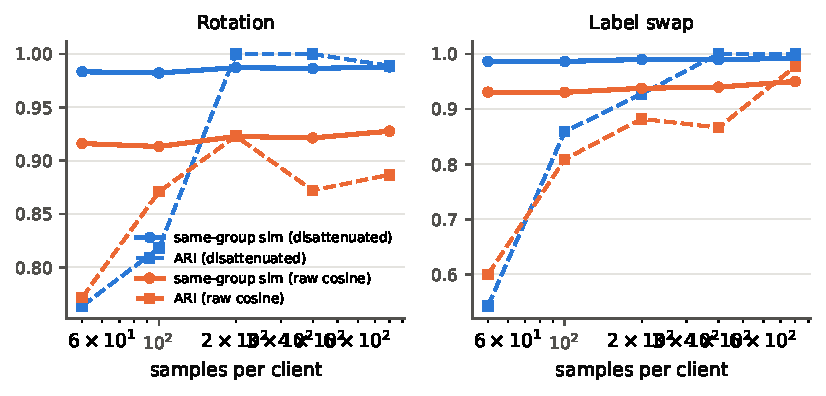
\includegraphics[width=0.85\linewidth]{../results/figures/sample_size.pdf}
\caption{Same-group similarity (solid) and ARI (dashed) as a function of the client size. Blue: disattenuated; orange: raw cosine.}\label{fig:size}
\end{figure}
\begin{figure}[!htbp]
\centering
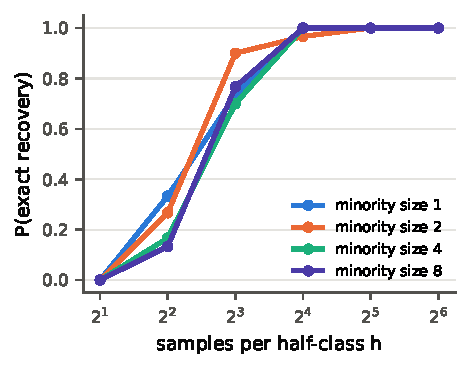
\includegraphics[width=0.45\linewidth]{../results/figures/theory_minority.pdf}
\caption{Synthetic validation of Corollary~\ref{cor:sc}: exact recovery of a minority group does not depend on its size.}\label{fig:thminority}
\end{figure}
\begin{table}[h]
\centering
\caption{Sensitivity to the shrinkage $\lambda$ at $\tau=0.8$: ARI / number of clusters (3 seeds, clustering step). For the label-only scenario the correct $K$ is 1.}\label{tab:lambda}
\small
\begin{tabular}{lccccc}
\toprule
Scenario & $\lambda=0.02$ & $\lambda=0.1$ & $\lambda=0.2$ & $\lambda=0.5$ & $\lambda=1.0$ \\
\midrule
Rotation & 1.00 / 4.0 & 1.00 / 4.0 & 1.00 / 4.0 & 1.00 / 4.0 & 0.98 / 4.0 \\
Label swap & 1.00 / 4.0 & 1.00 / 4.0 & 1.00 / 4.0 & 1.00 / 4.0 & 1.00 / 4.0 \\
Rotation + QS & 0.99 / 4.3 & 0.99 / 4.3 & 0.99 / 4.3 & 1.00 / 4.0 & 0.98 / 4.0 \\
Mixed + QS & 0.96 / 4.0 & 0.94 / 4.0 & 0.94 / 4.0 & 0.94 / 4.0 & 0.91 / 4.0 \\
Label skew only & 0.67 / 1.3 & 0.67 / 1.3 & 0.67 / 1.3 & 0.67 / 1.3 & 0.67 / 1.3 \\
Minority groups & 0.98 / 4.3 & 0.98 / 4.3 & 0.98 / 4.3 & 0.98 / 4.3 & 1.00 / 4.0 \\
\bottomrule
\end{tabular}
\end{table}


\subsection{Cost and scalability}\label{sec:cost}
Each client uploads its signature \emph{once}, about $1.2\times10^4$ floats with $p=1024$. The size is independent of the model dimension $d$; IFCA, by contrast, downloads $K$ models per client in \emph{every} round, and CFL/FL+HC cluster $d$-dimensional updates. Computing the signature takes 0.14--0.16\,s per client on one CPU core. Server-side clustering takes 0.05\,s for 40 clients and 2.3\,s for 320 clients, with ARI $\ge0.98$ at every scale.


\bibliographystyle{IEEEtranN}
\bibliography{refs}
\end{document}
